\begin{center}
	\Huge
	Tangentens ligning og ekstrema
\end{center}

\section*{Tangentens ligning}
\stepcounter{section}

Vi så sidst i tabellen over afledede funktioner, at $(e^x)' = e^x$, og at $(\ln(x))' = \frac{1}{x}$. Lad os se på et eksempel, hvor disse funktioner indgår.

\begin{exa}
	Vi får givet funktionen $f$ ved
	\begin{align*}
		f(x) = \ln(x),
	\end{align*}
	samt at $f$ har en tangent med ligningen $y = x + b$. Vi skal bestemme $b$.
	Vi starter med at differentiere $f$ for at finde $x_0$.
	\begin{align*}
		f'(x) = \frac{1}{x},
	\end{align*}
	hvilket giver os ligningen 
	\begin{align*}
		\frac{1}{x_0} = 1 \Leftrightarrow x_0 = 1.
	\end{align*}
	Vi bestemmer nu funktionsværdien $f(1)$ som
	\begin{align*}
		f(1) = \ln(1) = 0,
	\end{align*}
	og derfor fås ligningen 
	\begin{align*}
		y = x + b \Leftrightarrow 0 = 1 + b \Leftrightarrow b = -1.
	\end{align*}
	$b$ er altså lig $-1$, og tangentens ligning er derfor
	\begin{align*}
		y = x - 1.
	\end{align*}
\end{exa}

\section*{Ekstrema}
\stepcounter{section}

Vi talte i 1.g om ekstremumspunkter. Disse var punkter, der lokalt er maksimum eller minimum for en funktion. 

I mange sammenhænge er det en fordel at kunne bestemme \textit{toppunkter/maksima og minima} for en funktion $f$. Hvis $f$ er en differentiabel funktion, så kan vi udnytte differentialregning til at bestemme sådanne punkter. Et punkt, der enten er et maksimum eller et minimum kaldes et \textit{ekstremumspunkt}. 

Vi har følgende sætning:
\begin{setn}[Ekstremumspunkter]
	Lad $f$ være en differentiabel funktion. Hvis et punkt $P(x_0,f(x_0))$ er et ekstremumspunkt for $f$, så gælder der, at 
	\begin{align*}
		f'(x_0) = 0.
	\end{align*}
\end{setn}
Det er dog værd at bemærke, at vi ikke nødvendigvis har den omvendte implikation; hvis $f'(x_0)=0$, så er $(x_0,f(x_0))$ ikke nødvendigvis et ekstremumspunkt. Vi kalder sådanne for \textit{vandrette vendetangenter}. Vi kan se både en vandret vendetangent samt to ekstrema på Figur \ref{fig:ekstremavende}.


\begin{figure}[H]
	\centering
	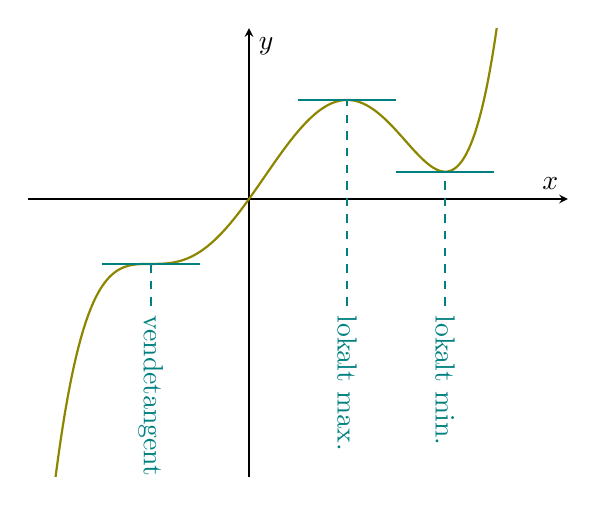
\begin{tikzpicture}
	\begin{axis}[
	axis lines = center, 
	xmin = -4.5, xmax = 6.5,
	ymin = -130, ymax = 80,
	xlabel = $x$, ylabel = $y$, 
	ticks = none,
	]
		\addplot[color = olive, thick, domain = -5:7, samples = 400] 
		{1/5*x^5-1/2*x^4-4*x^3+4*x^2+32*x };
		\node[color = teal, anchor = west, rotate = -90] at (axis cs: -2,-50) {vendetangent};
		\draw[color = teal, dashed, thick] (axis cs: -2,-50) -- (axis cs:-2,-152/5); 
		\node[color = teal, anchor = west, rotate = -90] at (axis cs: 2,-50) {lokalt max.};
		\draw[color = teal, dashed, thick] (axis cs: 2,-50) -- (axis cs:2,232/5); 
		\node[color = teal, anchor = west, rotate = -90] at (axis cs: 4,-50) {lokalt min.};
		\draw[color = teal, dashed, thick] (axis cs: 4,-50) -- (axis cs: 4,64/5); 
		\draw[color = teal, thick] (axis cs: -3,-152/5) -- (axis cs: -1,-152/5); 
		\draw[color = teal, thick] (axis cs: 1,232/5) -- (axis cs: 3,232/5); 
		\draw[color = teal, thick] (axis cs: 3,64/5) -- (axis cs: 5,64/5); 
	\end{axis}
	\end{tikzpicture}
	\caption{Forskellige ekstrema for en funktion samt vandrette tangenter}
	\label{fig:ekstremavende}
\end{figure}
\newpage
\begin{exa}
	Lad $f$ være givet ved
	\begin{align*}
		f(x) = x^3-6x^2+5.
	\end{align*}
	Vi ønsker at bestemme ekstrema for $f$. Vi differentierer derfor først $f$.
	\begin{align*}
		f'(x) = 3x^2-12x = 3x(x-4).
	\end{align*}
	Dette sættes nu lig $0$, og vi får
	\begin{align*}
		3x(x-4) = 0, 
	\end{align*}
	og ved hjælp af nulreglen ved vi, at $x=0$ eller $x = 4$. Vi bestemmer nu de tilhørende $y$-værdier og vi får
	\begin{align*}
		f(0) = 5
	\end{align*}
	og 
	\begin{align*}
		f(4) &= 4^3 - 6\cdot 4^2+5\\
		&= 64-96+5\\
		&= -27.
	\end{align*}
	Vi har derfor en vandret tangent i $P(0,5)$ og $Q(4,-27)$. For at bestemme, om det er et ekstremumspunkt, så tegner vi grafen. Denne kan ses af Figur \ref{fig:ekstrema}
	\begin{figure}[H]
		\centering
		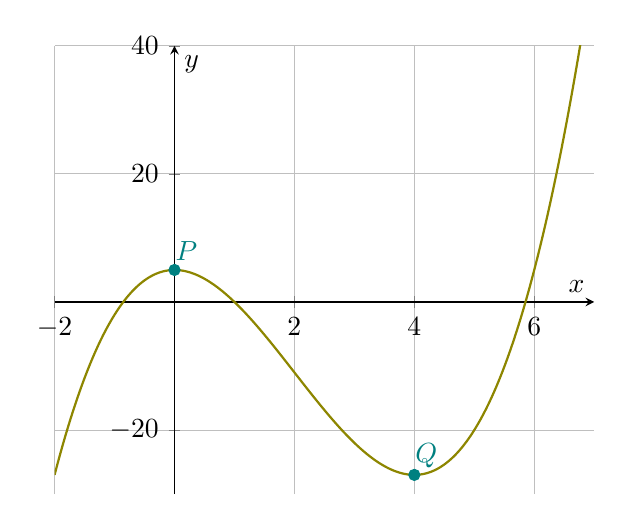
\begin{tikzpicture}
			\begin{axis}[axis lines = middle,
			xmin = -2, xmax = 7,
			ymin = -30, ymax = 40,
			xlabel = $x$, 
			ylabel = $y$,
			grid = both]
				\addplot[color = olive, samples = 200, domain = -2:7, thick] {x^3-6*x^2+5};
				\filldraw[color = teal] (axis cs:0,5) circle (2pt);
				\filldraw[color = teal] (axis cs:4,-27) circle (2pt);
				\node[color = teal] at (axis cs: 0.2,8) {$P$};
				\node[color = teal] at (axis cs: 4.2,-24) {$Q$};
			\end{axis}
		\end{tikzpicture}
		\caption{Graf for funktionen $f$.}
		\label{fig:ekstrema}
	\end{figure}
\end{exa}
Af Figur \ref{fig:ekstrema} kan vi se, at punkterne $P$ og $Q$ er ekstremumspunkter. $P$ er et \textit{lokalt maksimum} og $Q$ er et \textit{lokalt minimum}. Vi kan også se, at $f$ ikke har nogle 
\textit{globale ekstrema}.




\subsection*{Opgave 1 (Med hjælpemidler)}
Bestem tangentens ligning for følgende funktioner i det angivne punkt. Tegn desuden grafen for funktionen samt tangenten i Maple.
\begin{align*}
	&1) \ f(x) = 2\ln(x) - x^2, \ P(1,f(1)) &&2) \ f(x) = \sqrt{2x} + e^{2x}, \ P(4,f(4))\\
	&3) \ f(x) = 3x^4-6x^2+5, \ P(3,f(3)) &&4) \ f(x) = x^{1.6}, \ P(-3	,f(-3))\\
\end{align*}

\subsection*{Opgave 2 (Med hjælpemidler)}
Funktionen $f$ er givet ved
\begin{align*}
	f(x) = \ln(x) - \frac{1}{2}x^2 + \frac{1}{10}x^3.
\end{align*}
\begin{enumerate}[label=\roman*)]
	\item Bestem tangentens ligning for $f$ i punktet $P(0.5,f(0.5))$.
\end{enumerate}
Det oplyses, at $f$ har en anden tangent, der er parallel med tangenten i punktet $P$.
\begin{enumerate}[label=\roman*)]
	\setcounter{enumi}{1}
	\item Bestem ligningen for denne tangent.
\end{enumerate}

\subsection*{Opgave 3 (Med hjælpemidler)}
To andengradspolynomier $p$ og $q$ er givet ved
\begin{align*}
	p(x) = 2x^2+bx+1 \quad \text{og} \quad q(x) = -x^2+3x-5.
\end{align*}
\begin{enumerate}[label=\roman*)]
	\item Bestem de værdier for tallet $b$ så tangenten til $p$ i punktet $P(2,P(2))$ er en tangent til $q$. Tegn desuden grafen for $p$ og $q$ samt tangenterne i Maple.
\end{enumerate}

\subsection*{Opgave 4}
Vis, at skæringspunktet med $y$-aksen for tangenten til et andengradspolynomium $p$ givet ved
\begin{align*}
	p(x) = ax^2 + bx + c
\end{align*}
i et punkt $P(x_0,p(x_0))$ ikke afhænger af værdien af $b$.

\newpage

\subsection*{Opgave 4}

Bestem ekstremumspunkter for følgende funktioner. Løs først ligningen $f'(x)=0$ og tegn derefter grafen for funktionen.  Afgør til sidst, om der er tale om globale maksimum/minimum eller lokale maksimum/minimum.

\begin{align*}
	&1) \ f(x) = -x^2+10    &&2) \  f(x) = x^3     \\
	&3) \  f(x) = x^4-8x^2   &&4) \ f(x) = \ln(x) - \frac{1}{2}x^2      \\
	&5) \  f(x) = 6\sqrt{x}-x^3    &&6) \   f(x) = \frac{16}{x} +x^2    \\
	&7) \  f(x) = x^5-10x^4   &&8) \ f(x) = \frac{8}{x} + 2x      \\
\end{align*}

\subsection*{Opgave 5}
En funktion $f$ er givet ved
\begin{align*}
	f(x) = \frac{1}{3}x^3 - bx^2.
\end{align*}
\begin{enumerate}[label=\roman*)]
	\item Bestem $b$ så $f$ har et ekstremum i punktet $P(2,f(2))$.
	\item Bestem $b$ så $f$ har et ekstremum i punktet $Q(4,f(4))$.
\end{enumerate}

\subsection*{Opgave 6}
En funktion $g$ er givet ved
\begin{align*}
	g(x) = ax^3 - 5x^2 + 21x.
\end{align*}
\begin{enumerate}[label=\roman*)]
	\item Bestem tallet $a$, så funktionen $g$ har et ekstremum i punktet $P(3,g(3))$.
\end{enumerate}



\subsection*{Opgave 7}
\begin{enumerate}[label=\roman*)]
	\item Tegn funktionen $\sin(x)$ på intervallet $[-10,10]$.
	\item Hvor mange ekstrema har $\sin(x)$ på dette interval og hvilken type har de?
	\item Bestem ekstrema for $\sin(x)$.
\end{enumerate}

\subsection*{Opgave 8}
\begin{enumerate}[label=\roman*)]
	\item Hvad sker der, hvis I differentierer $\cos(x)$ to gange?
	\item Hvad sker der, hvis I differentierer $\sin(x)$ to gange?
	\item Hvad sker der, hvis I differentierer $\cos(x)$ fire gange?
	\item Hvad sker der, hvis I differentierer $\sin(x)$ fire gange?
\end{enumerate}